


\section{Results}



\subsection{Previous Results}

As mentioned previously, this project is a continuation of a project done over the previous year in
which we developed a method to use pulsar timing data to constrain our models. The final results of
that project were a set of models that accurately reproduce all observables and fully incorporated
the pulsar data. The best fit parameters of this set of models are listed in Table
\ref{tab:parameters_nobin}. Figure \ref{fig:nobin_obs_panel} shows the model fits to most of
the observables while Figure \ref{fig:nobin_mass_fun} shows the fit to the stellar mass function
data.

One of the most interesting results of the previous project was the models' ability to constrain the
black hole content within 47\,Tuc. Figure \ref{fig:prev_nobin_BH_dists} shows the distribution of
black hole mass and number in  our set of best fit models. Both the total mass and number are quite
well contained especially in comparison to the previous constraints in the literature \citep[see
	e.g.][]{Henault-Brunet2020,Weatherford2019}.


\begin{table}
	\centering
	\caption{Best fit parameters with $1-\sigma$ intervals.}
	\begin{tabular}{l l}

		\hline
		Parameter                 & Value                     \\
		\hline
		$\Phi_0$                  & $6.444^{+0.137}_{-0.126}$ \\
		$M/10^6 \mathrm{M}_\odot$ & $0.864^{+0.009}_{-0.009}$ \\
		$r_h / pc$                & $6.612^{+0.069}_{-0.067}$ \\
		$\log{r_a / pc}$          & $1.425^{+0.039}_{-0.035}$ \\
		$g$                       & $1.264^{+0.064}_{-0.072}$ \\
		$\delta$                  & $0.397^{+0.019}_{-0.020}$ \\
		$s^2$                     & $0.019^{+0.059}_{-0.013}$ \\
		$F$                       & $2.972^{+0.019}_{-0.039}$ \\
		$\alpha_1$                & $0.468^{+0.047}_{-0.041}$ \\
		$\alpha_2$                & $1.178^{+0.053}_{-0.057}$ \\
		$\alpha_3$                & $2.117^{+0.039}_{-0.038}$ \\
		$BH_{ret} (\%)$           & $0.128^{+0.084}_{-0.061}$ \\
		$d$                       & $4.433^{+0.021}_{-0.023}$ \\
		\hline
	\end{tabular}
	\label{tab:parameters_nobin}
\end{table}

\begin{figure}
	\centering
	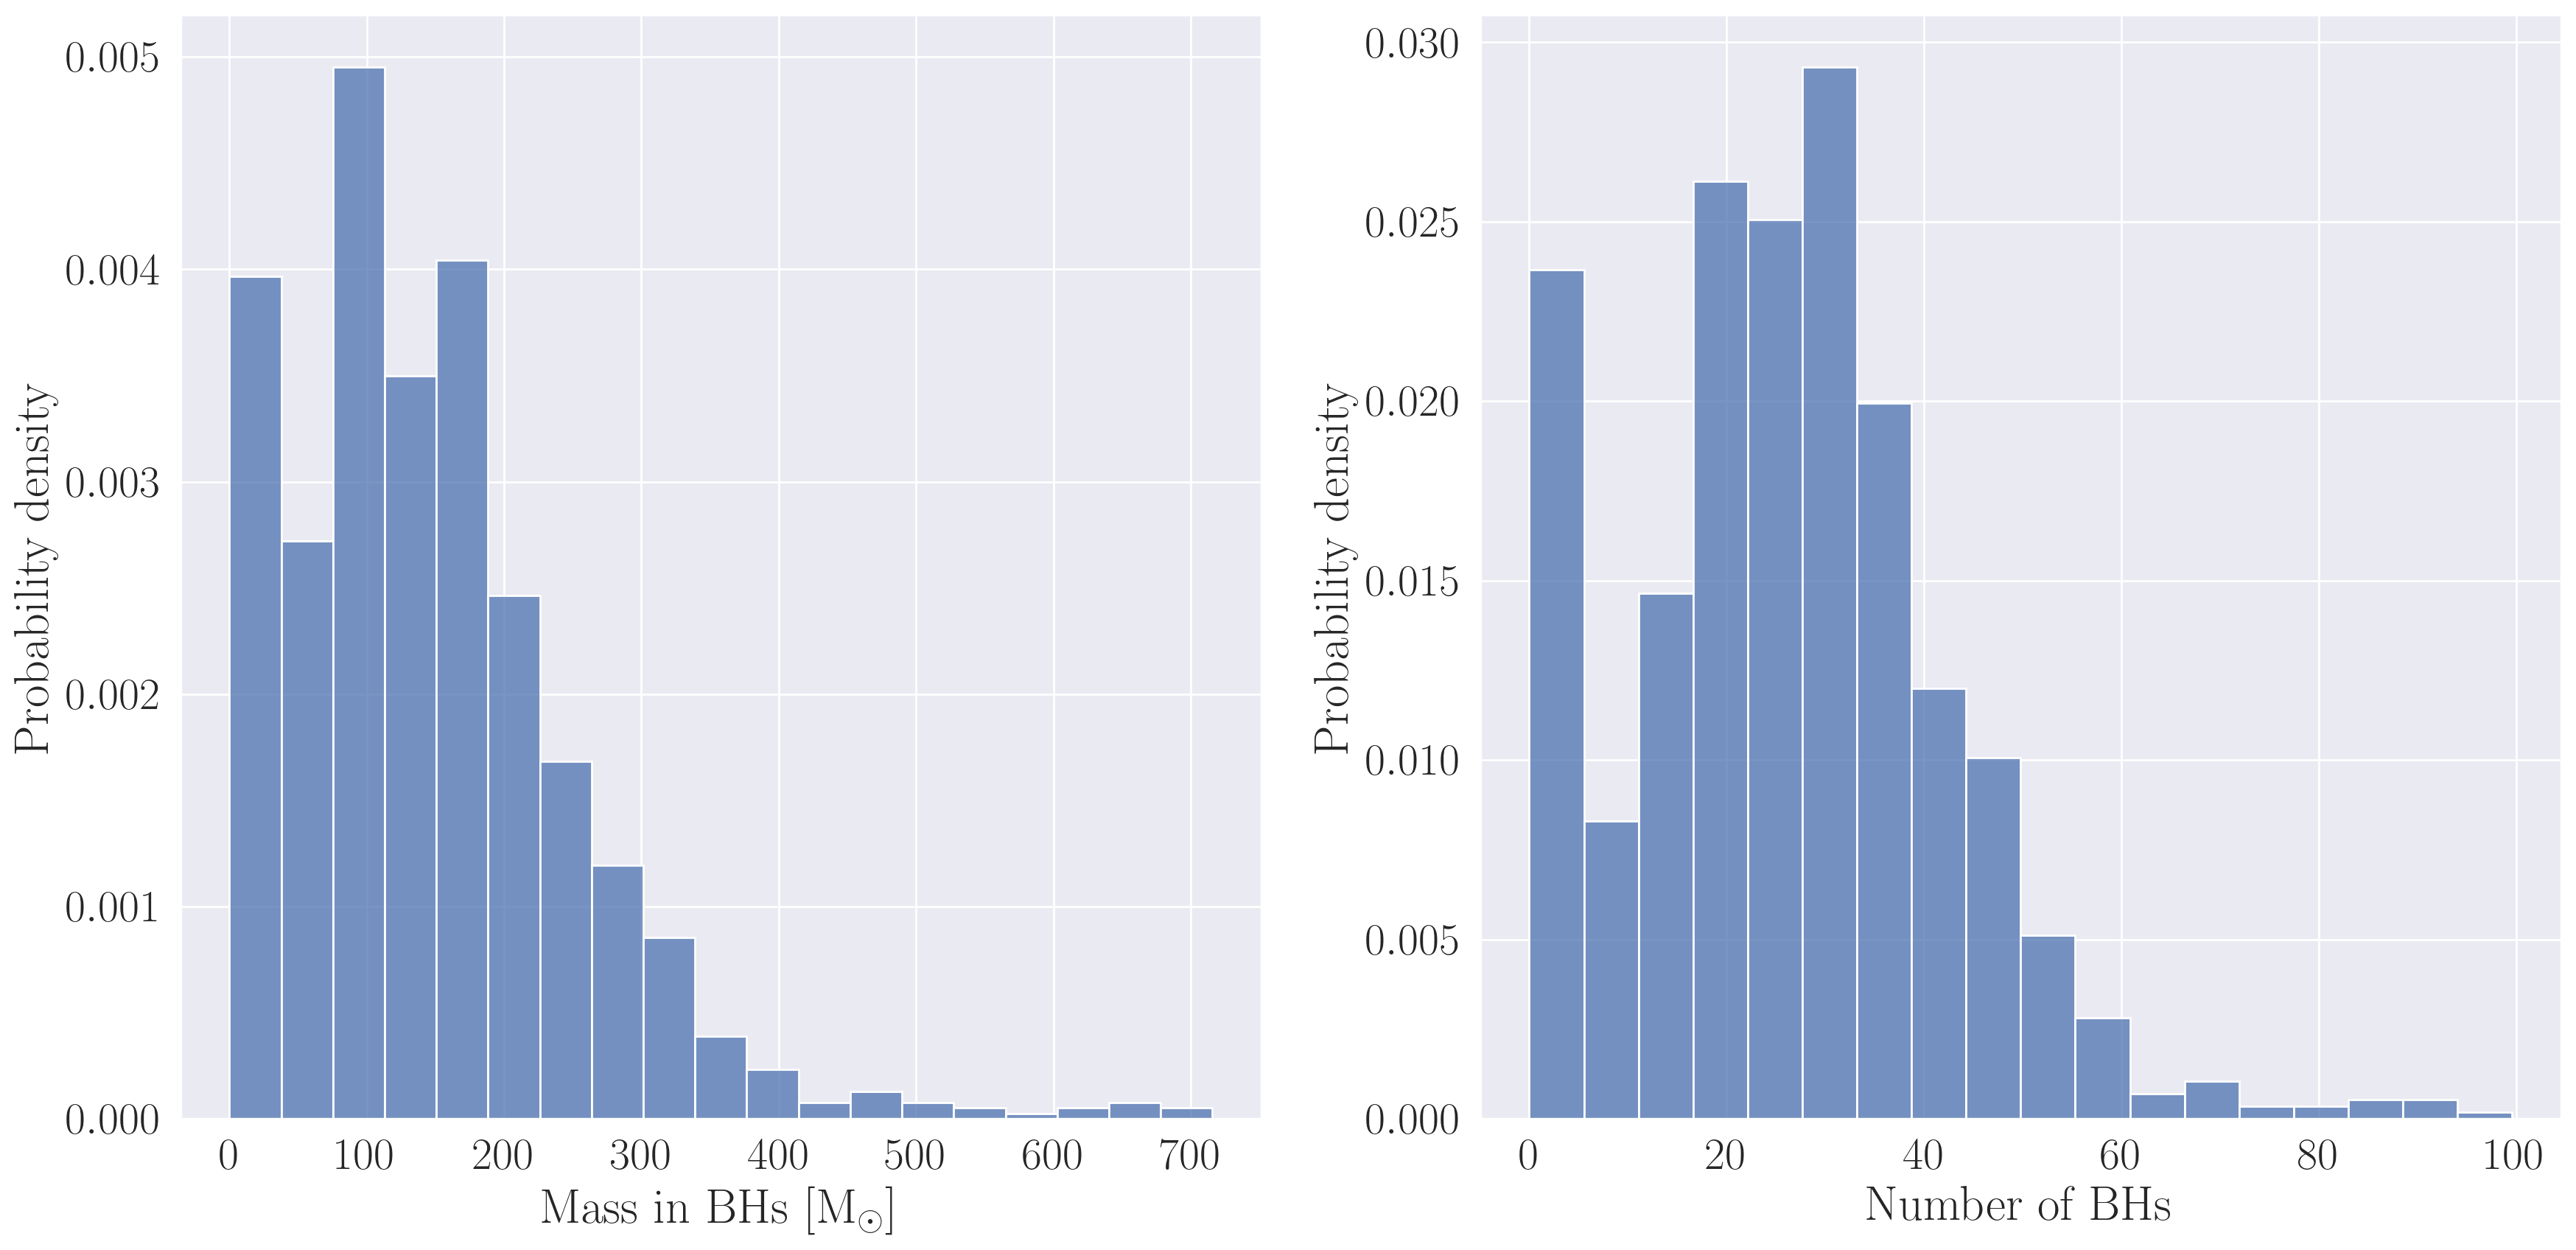
\includegraphics[width=0.8\textwidth]{figures/prev_nobin/BH_dists.png}
	\caption{BH distributions}
	\label{fig:prev_nobin_BH_dists}
\end{figure}


\subsection{Low Binary Fraction}
\ps{Describe the results for the low binary fraction model.}

In the low binary fraction case, the model is similar to the model without binaries. Maybe?

\ps{Figures with usual model quantities, also the binary mass histogram and the density profiles}


\begin{figure}
	\begin{center}
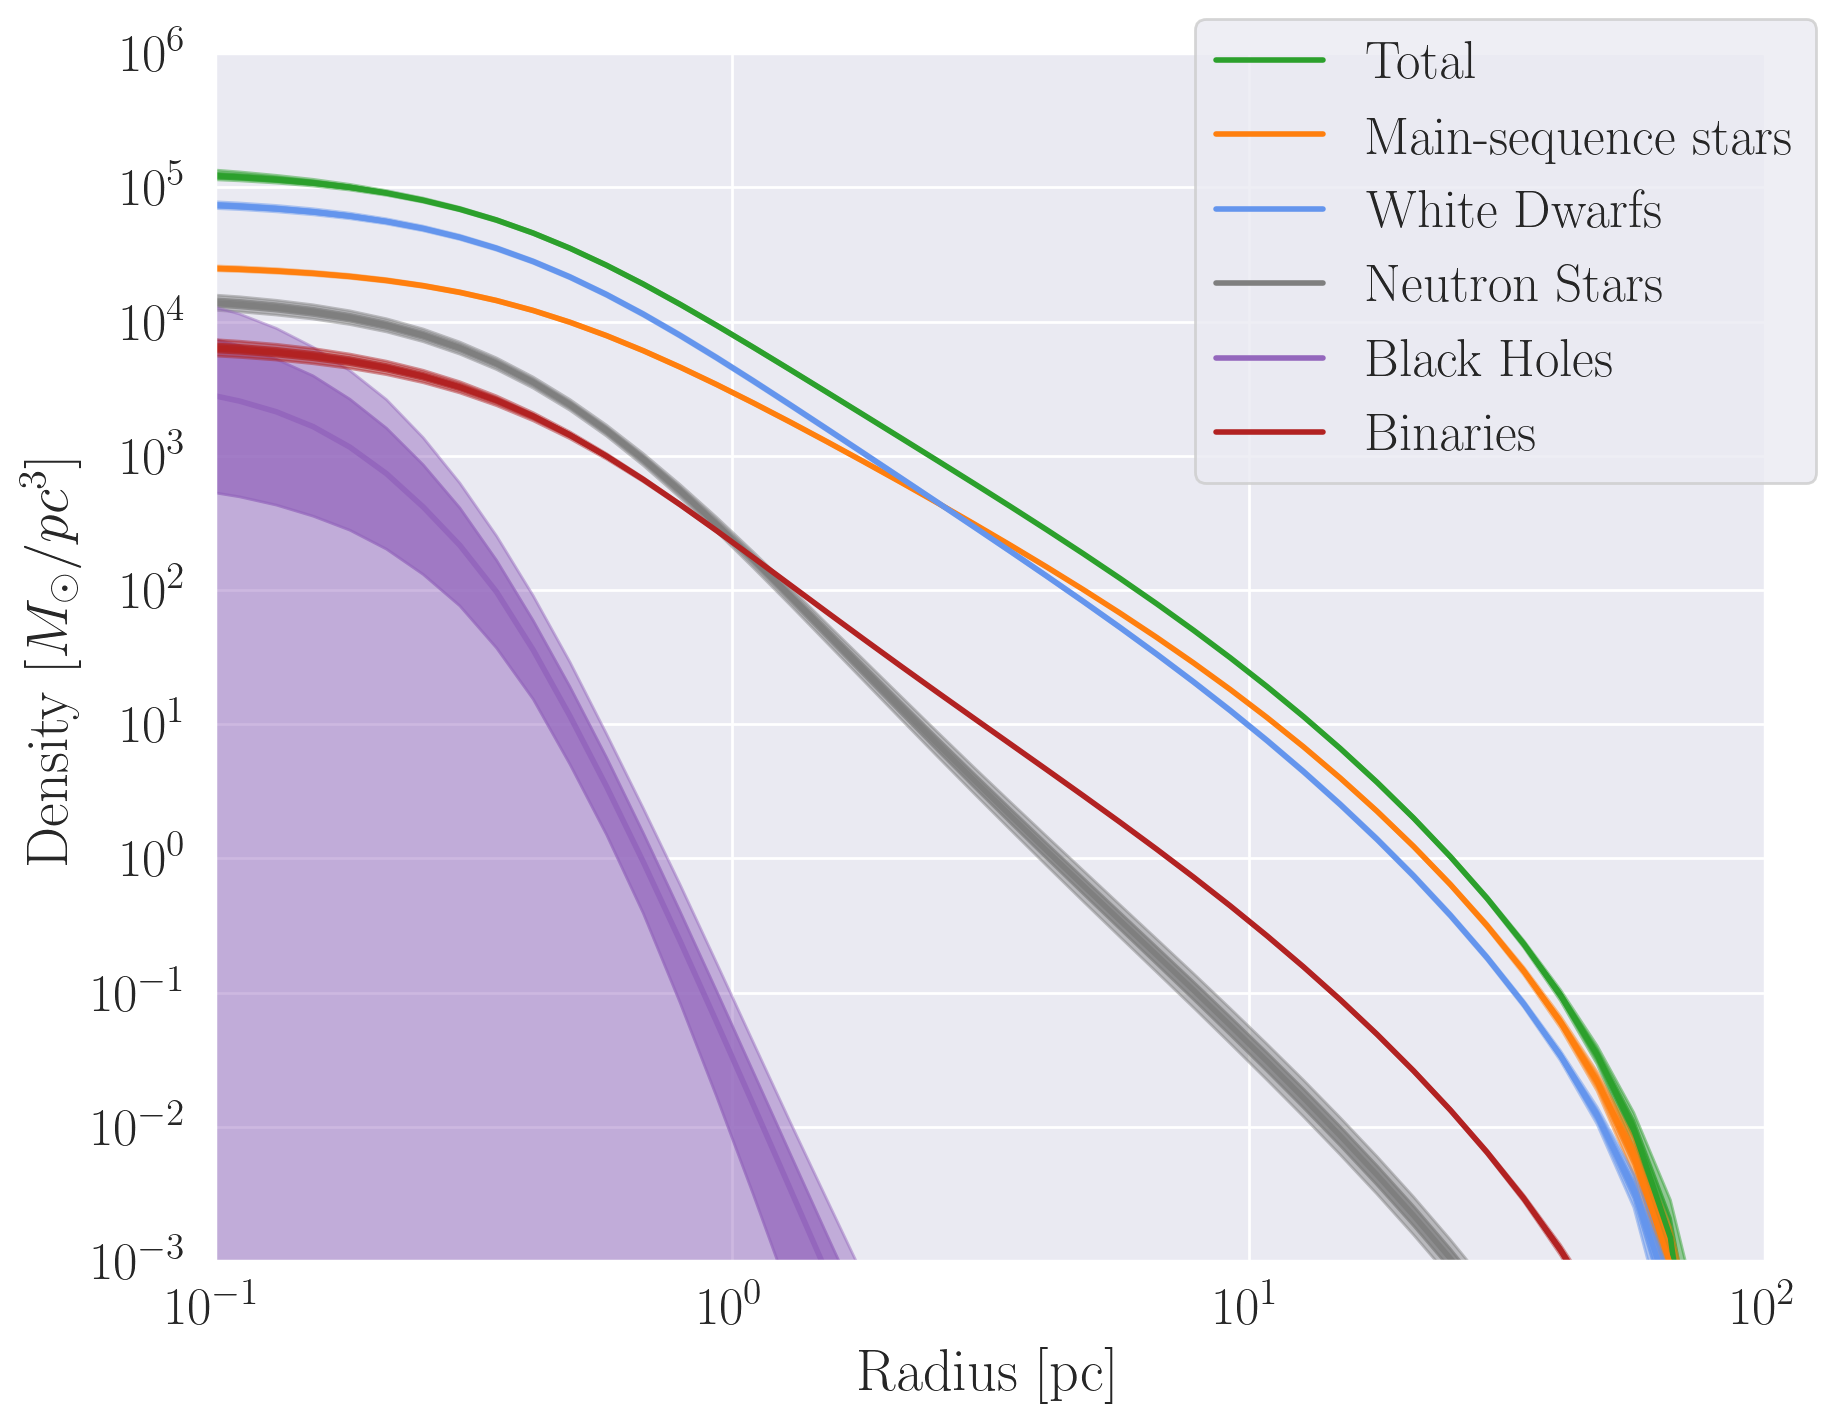
\includegraphics[width=0.9\textwidth]{figures/low_bin_model/density.png}
	\end{center}
\caption{Density Profiles}
	\label{fig:low_bin_model_densities}
\end{figure}

\begin{figure}
	\begin{center}
		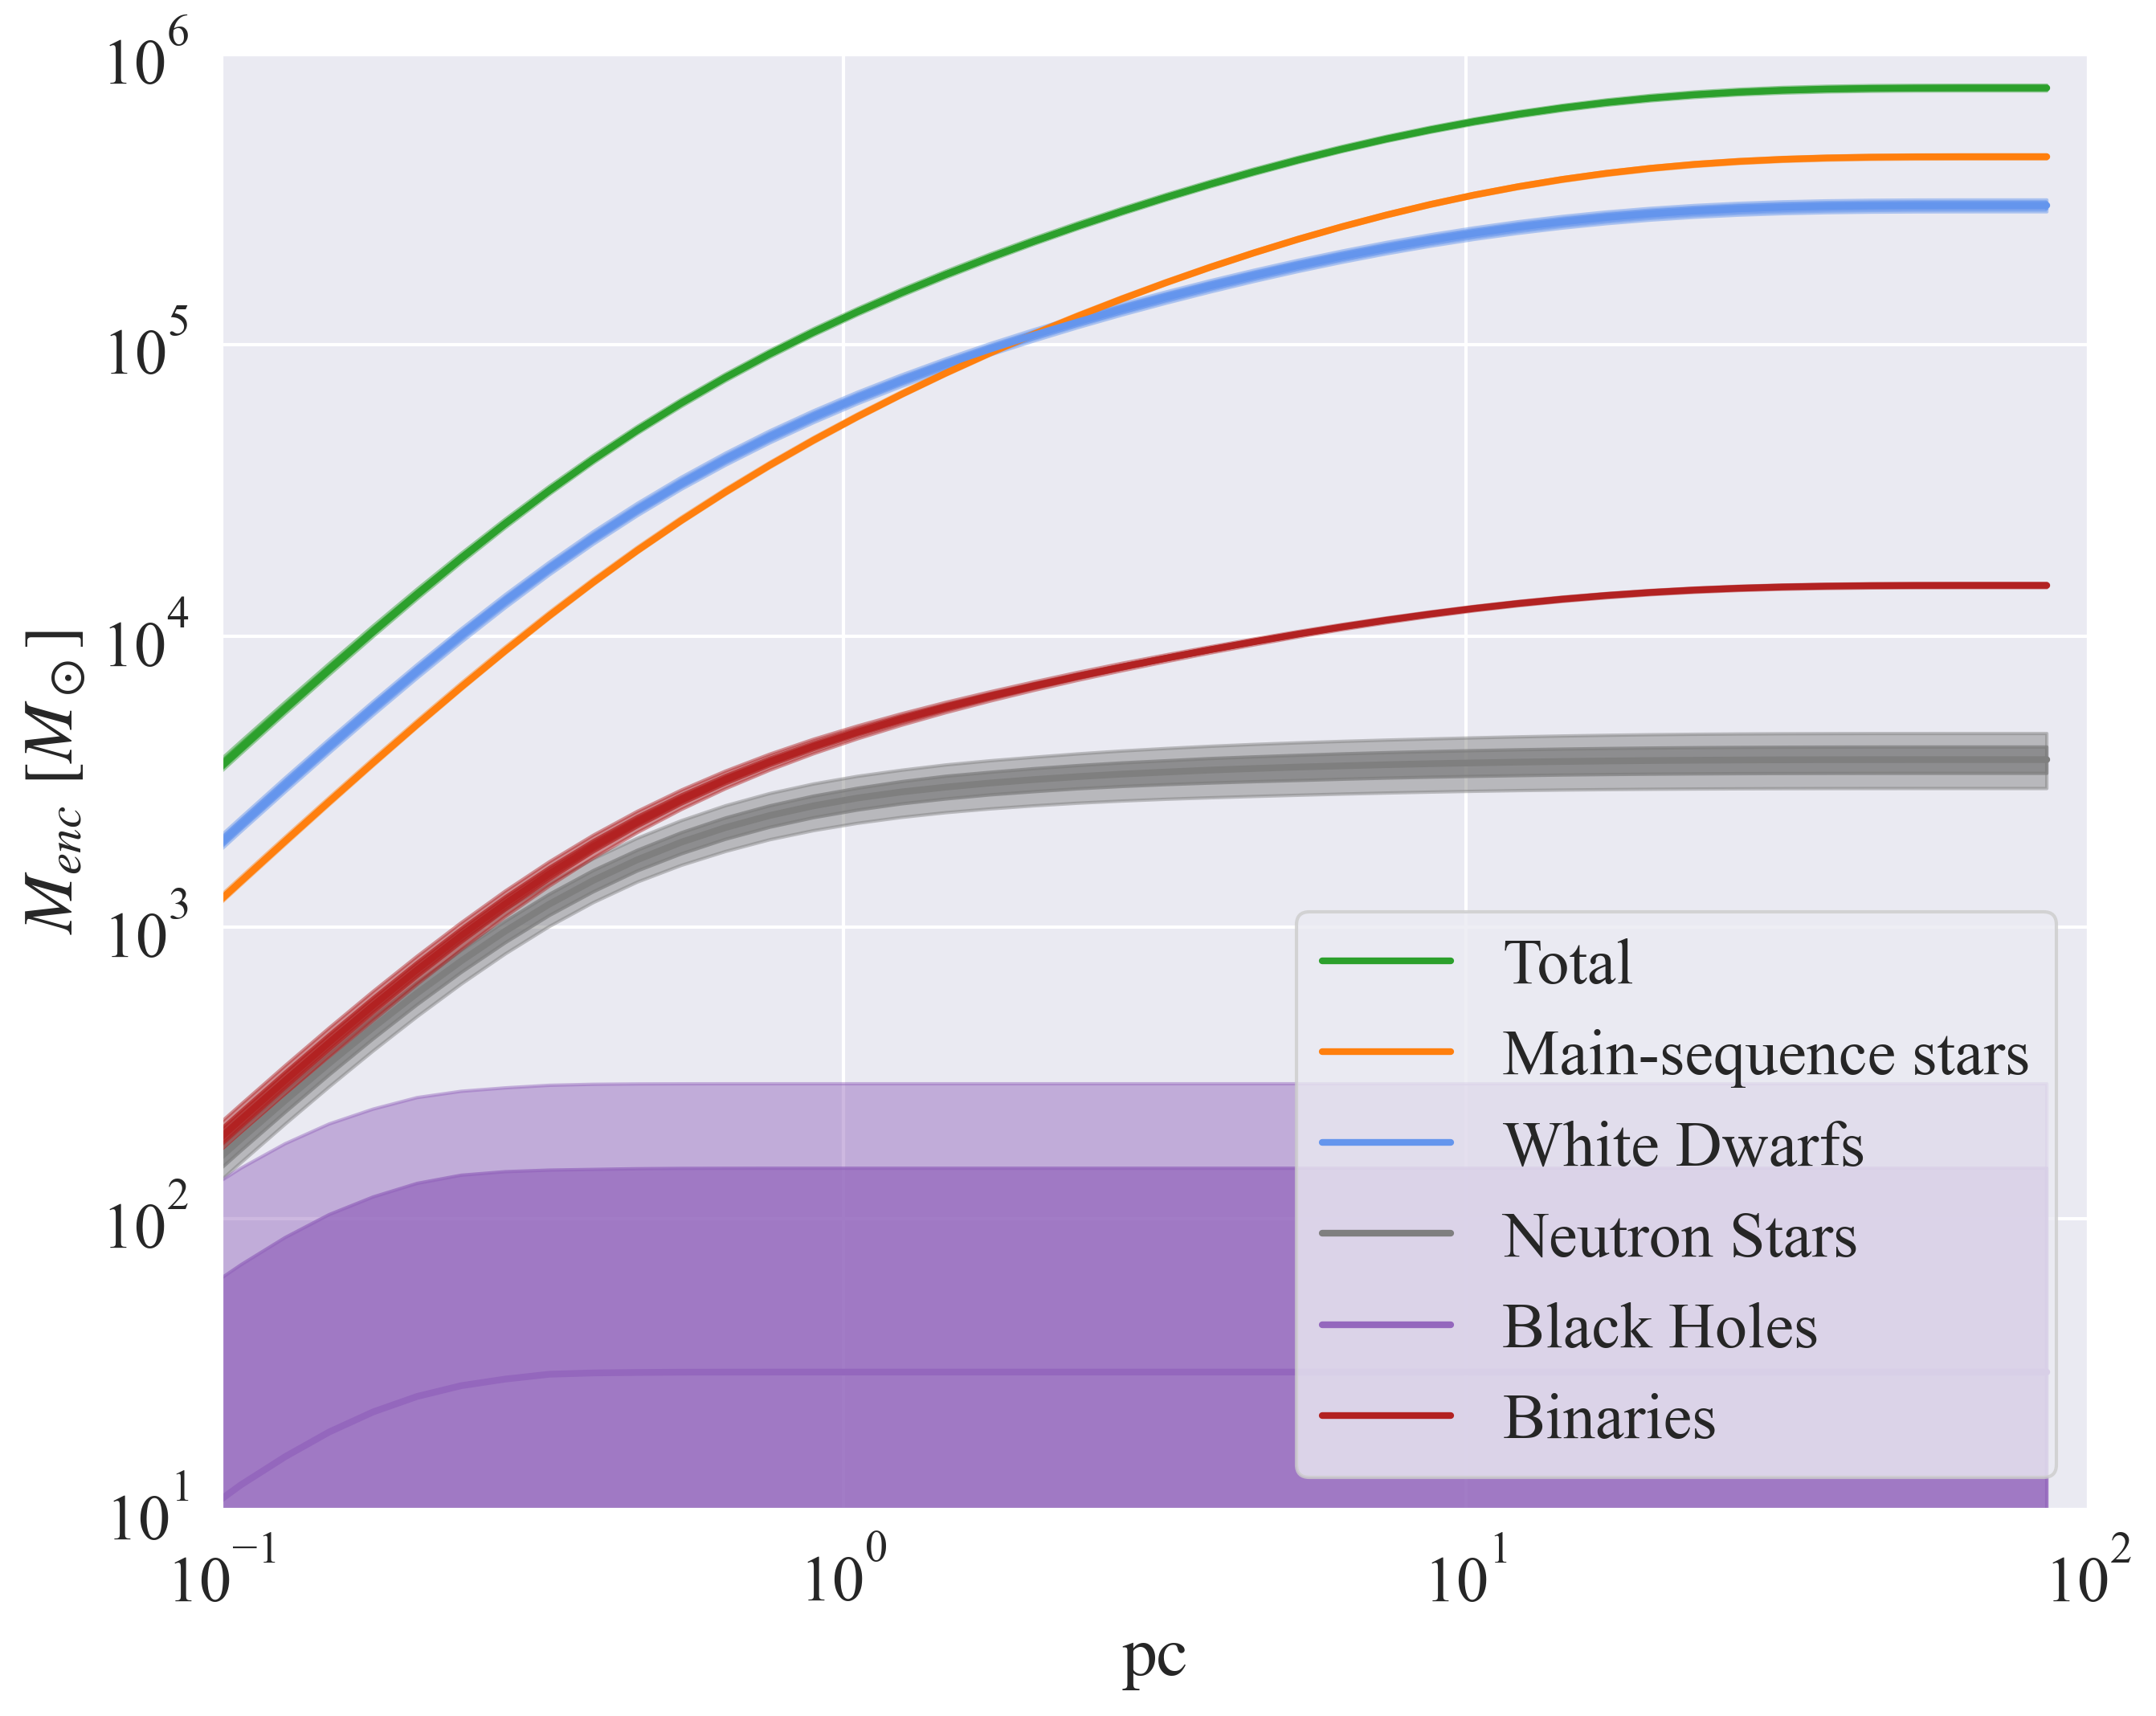
\includegraphics[width=0.9\textwidth]{figures/low_bin_model/mass_enc.png}
	\end{center}
	\caption{Density Profiles}
	\label{fig:low_bin_model_enclosed_mass}
\end{figure}

\begin{figure}
	\begin{center}
		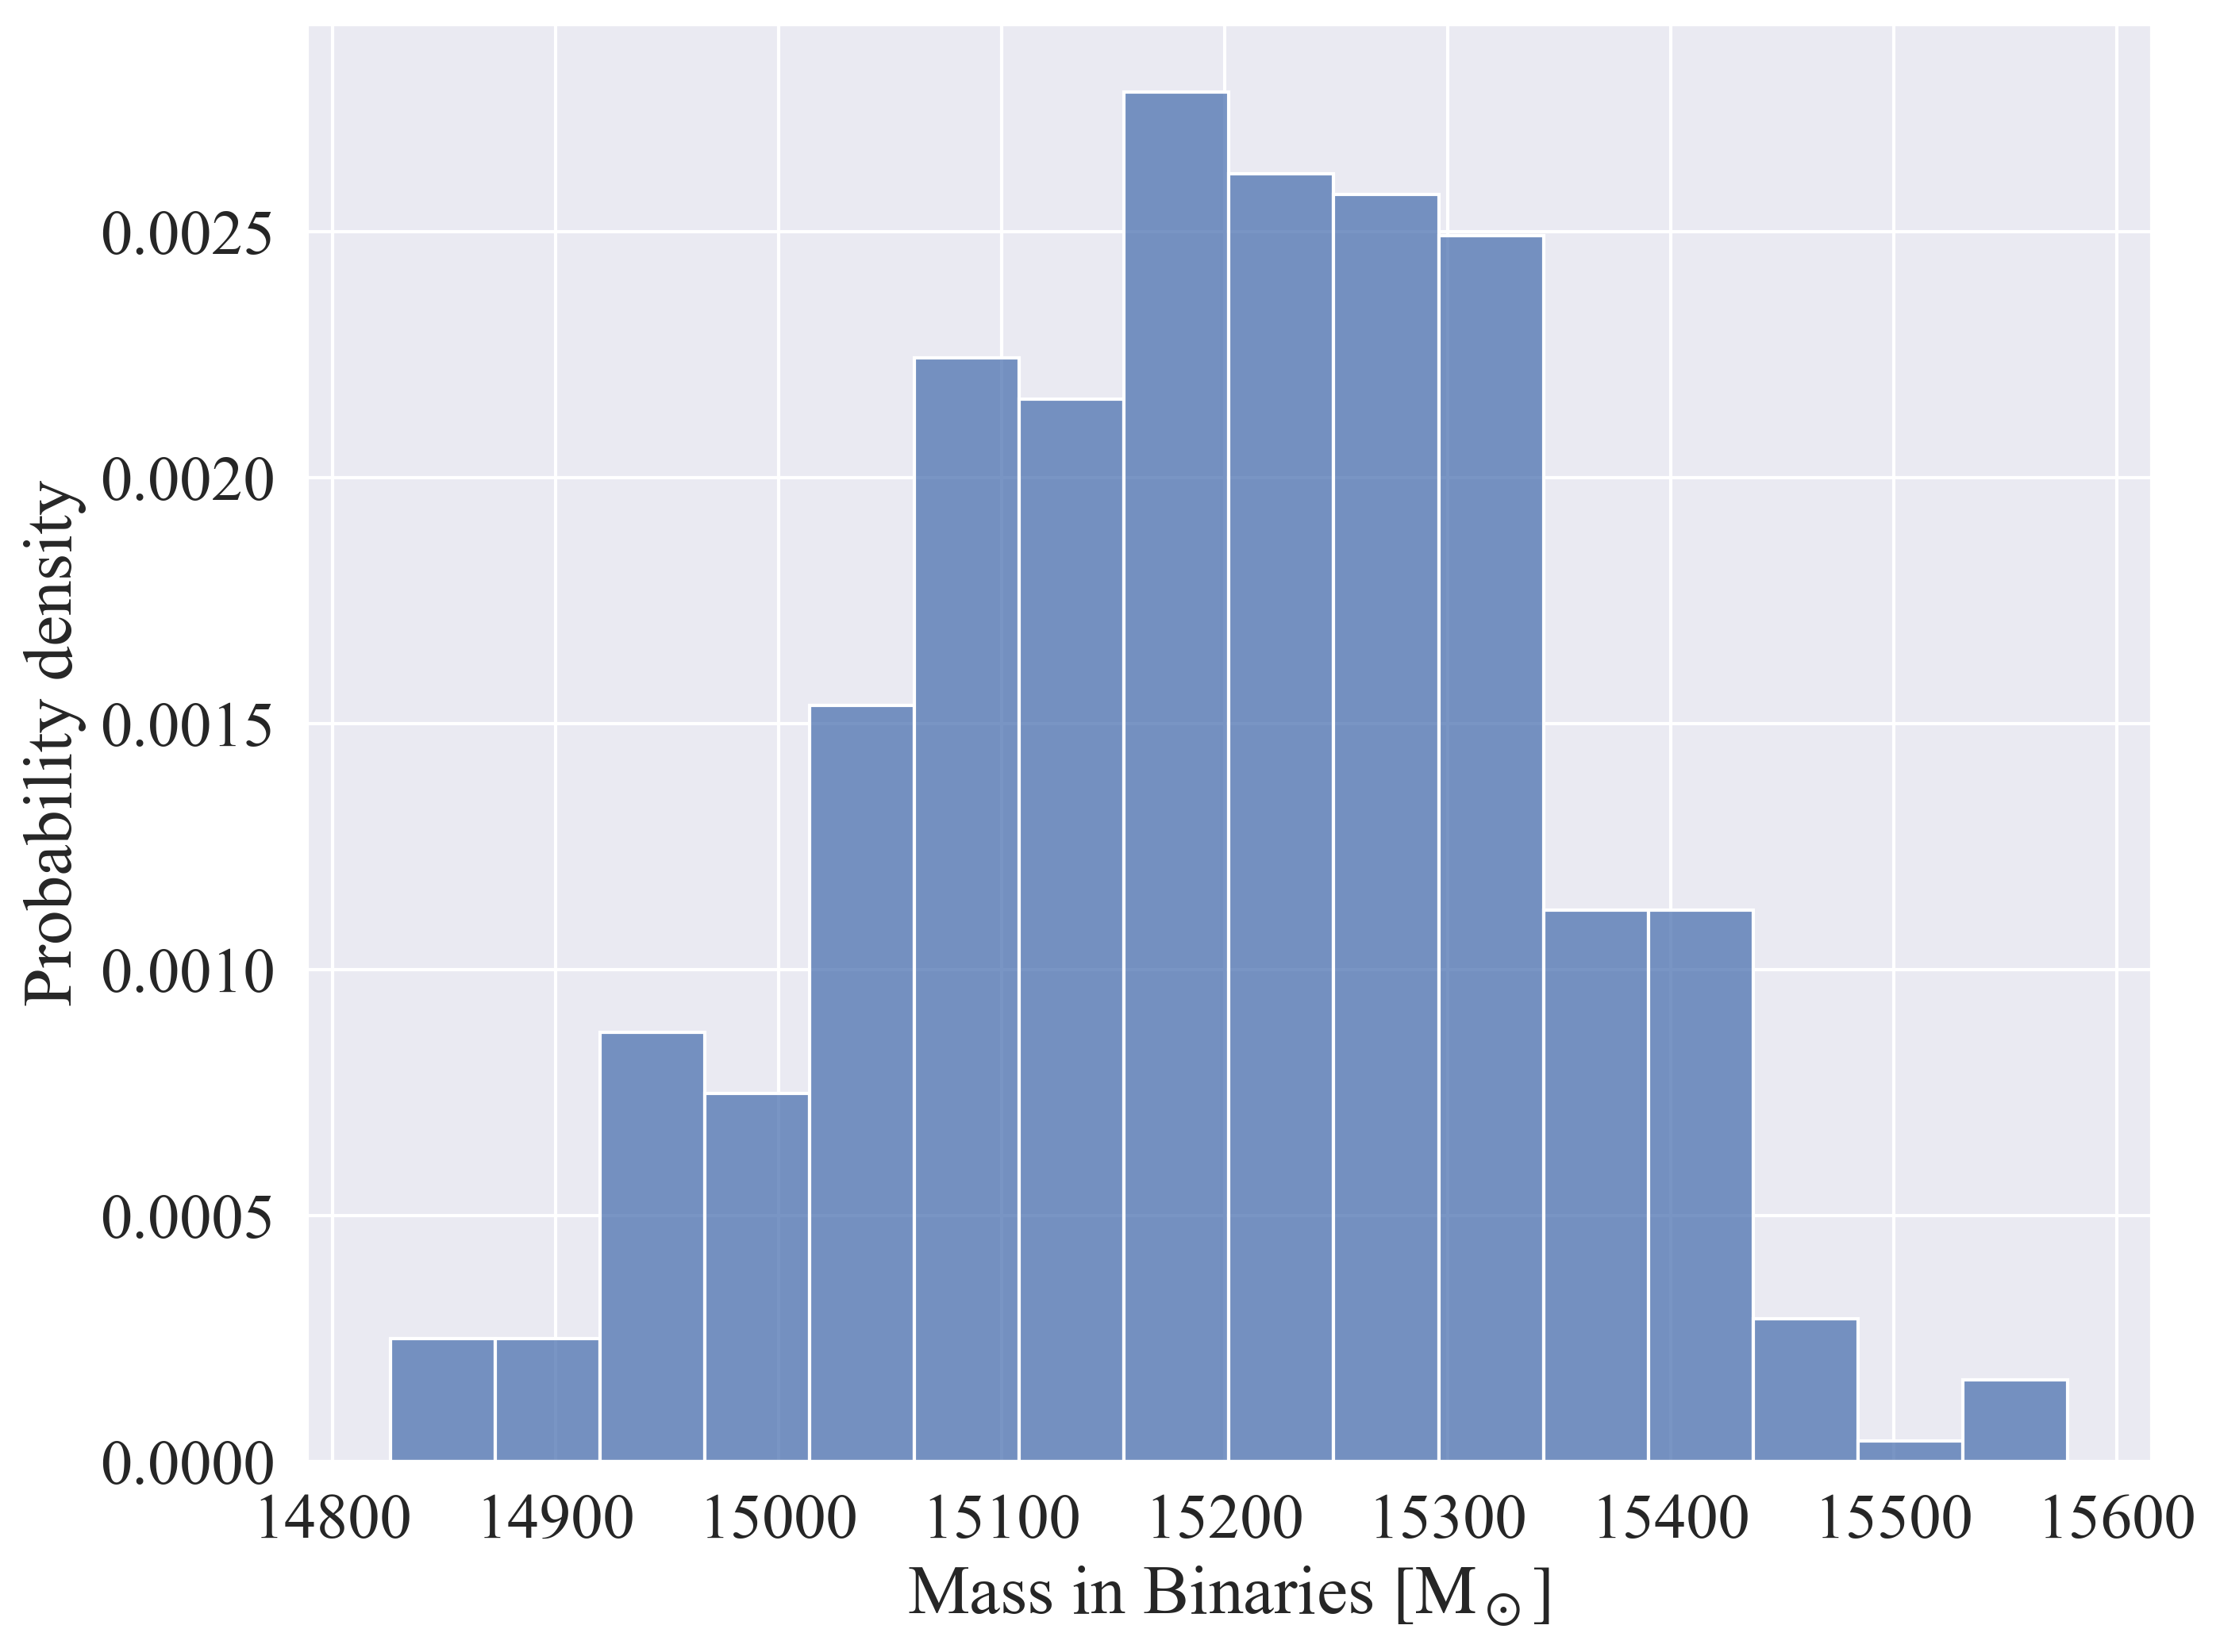
\includegraphics[width=0.9\textwidth]{figures/low_bin_model/binary_mass.png}
	\end{center}
	\caption{Total mass in binaries}
	\label{fig:low_bin_model_binary_mass}
\end{figure}

\begin{figure}
	\begin{center}
		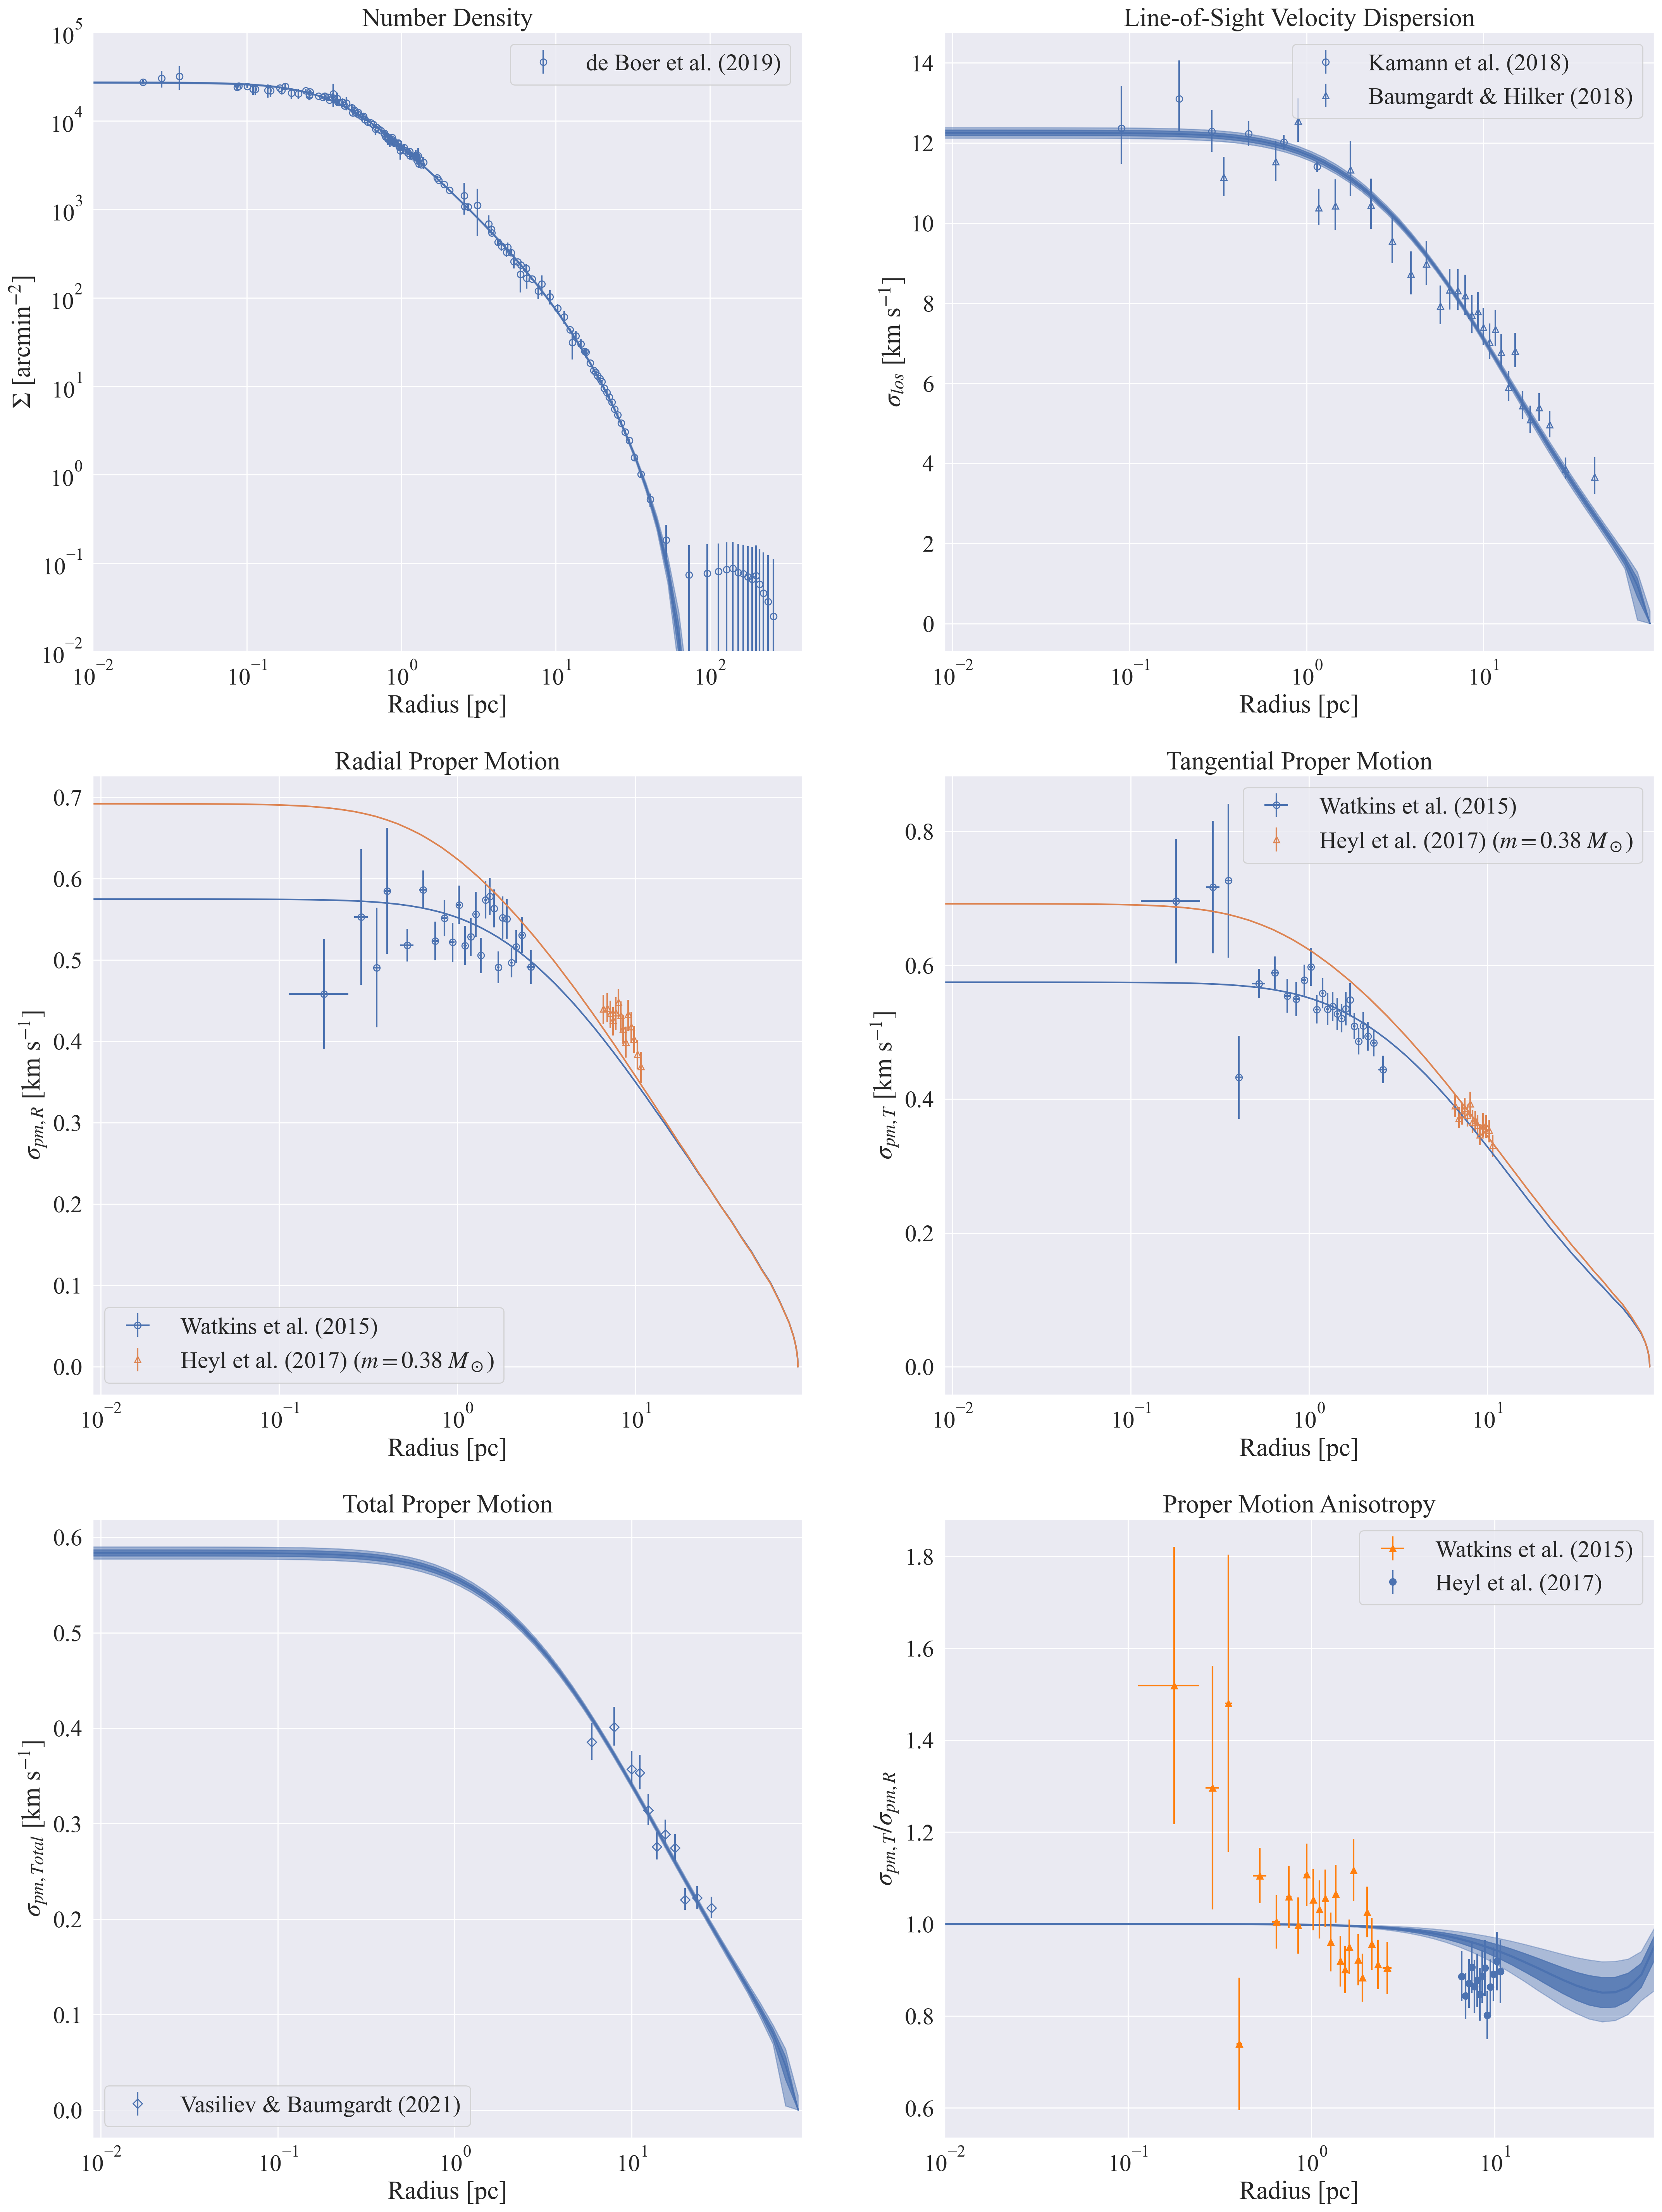
\includegraphics[width=0.9\textwidth]{figures/low_bin_model/obs_panel.png}
	\end{center}
	\caption{Observables}
	\label{fig:low_bin_model_obs_panel}
\end{figure}


\begin{figure}
	\begin{center}
		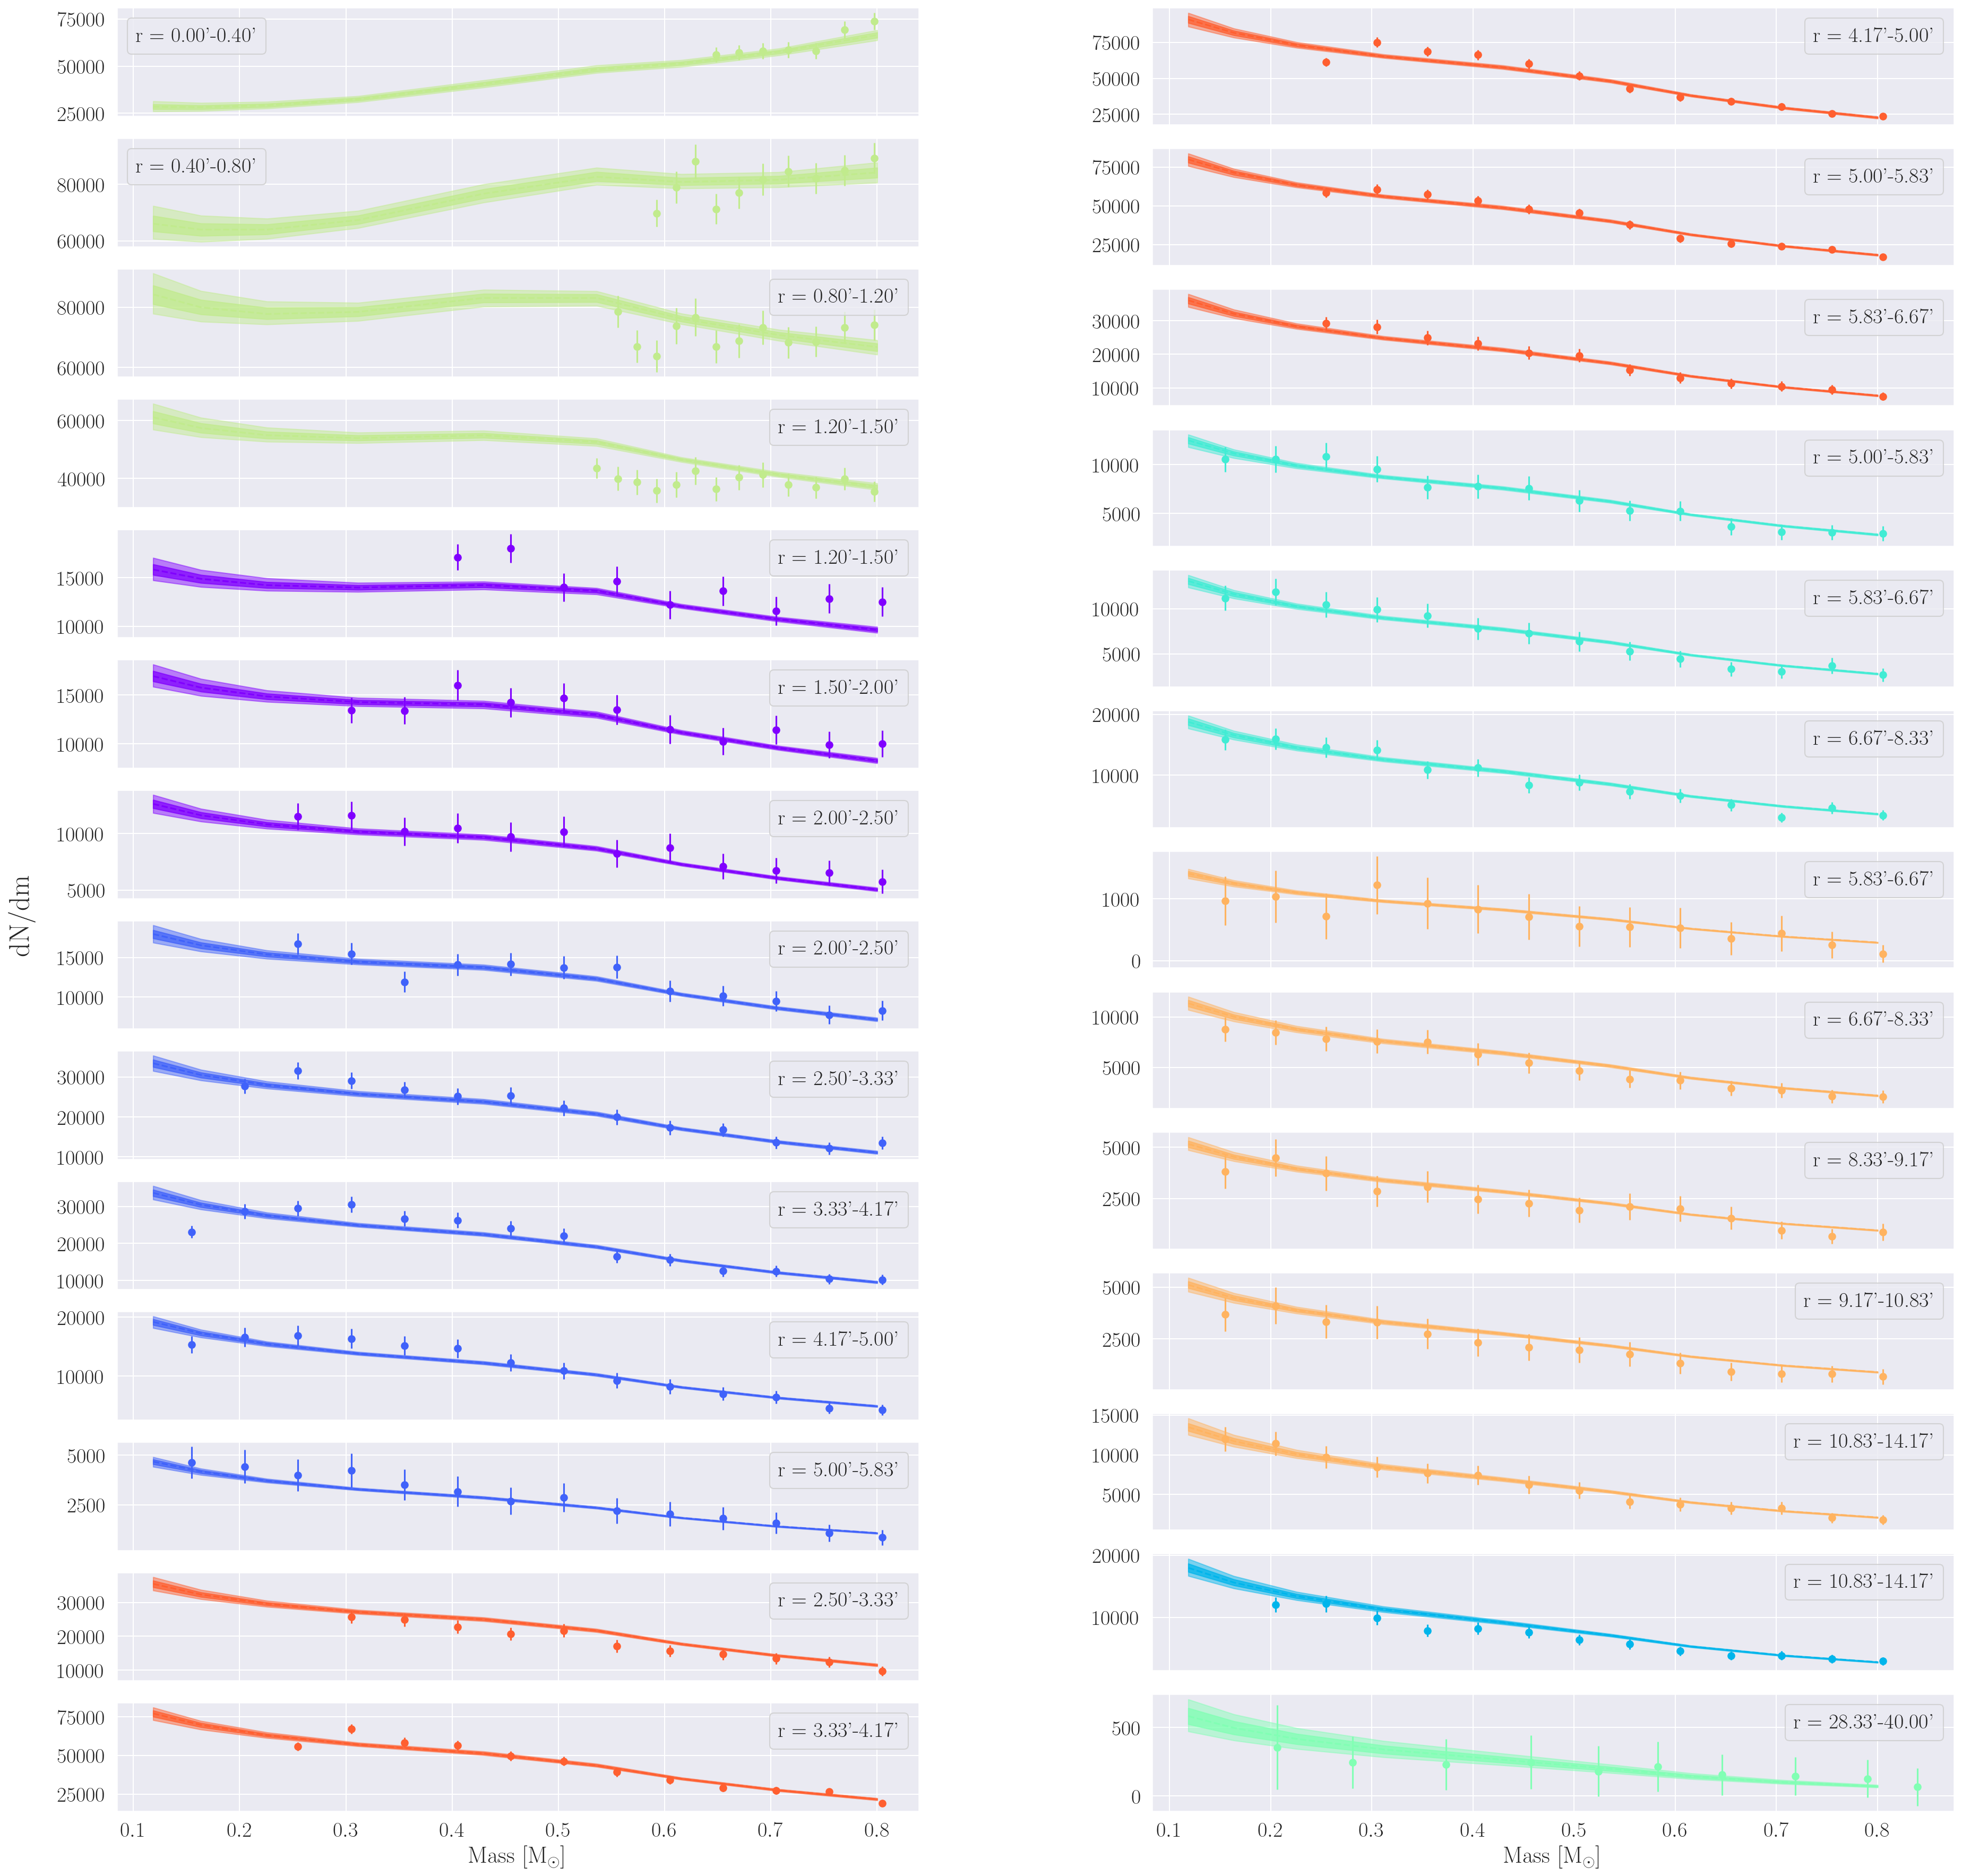
\includegraphics[width=\textwidth]{figures/low_bin_model/mass_fun.png}
	\end{center}
	\caption{Mass function}
	\label{fig:low_bin_model_mass_fun}
\end{figure}








\subsection{High Binary Fraction}
\ps{Describe the results for the high binary fraction model.}

\ps{Figures with usual model quantities, also the binary mass histogram and the density profiles}







\section{Discussion}

\subsection{The effects of the binaries}

Generally mimic a small population of remnants?









\subsection{Conclusion}

\ps{Implications for past/future work}

\ps{Do binaries in df models actually matter?}








\subsection{Future Work}

We're only looking at binaries in main sequence stars. WD binaries are probably a bigger effect, but
we have no data at all to constrain those quantities, so we ignore them. Maybe looking at N-body or
MC models could give some useful constraints.

Would be nice to look at a cluster where we know there is a larger binary population (NGC3201)and
fit with and without binaries to see what the effects are.